% Template PNSAC newsletter - Article
% Language: Latex
%

% Head

\title{Conservator's Corner}
%\subtitle{PNS 2016 Status Update}
\author{R\'{e}jean Demers\\ Conservator\\ Canadian Aviation and Space Museum}

\maketitle

\textbf{Stabs and Tail Feathers}

Some tasks are easier than others, this is not a simple one. North Star S/N:
122, registration 17515, was delivered to the National Aeronautical collection
in 1965, intact and airworthy. After spending 39 years parked on the tarmac,
awaiting restoration, the condition of its flight control surfaces had become
less a statement of endurance and more a sad result of the elements. 

\begin{figure}[httb]
   \vspace{2em}
   \centering
   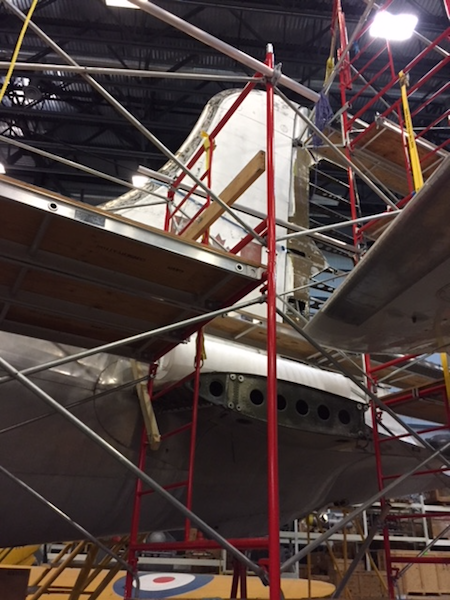
\includegraphics[scale=0.5]{IMG_0705-scaled.png}
   \caption*{\small \em Scaffold erected next to North Star to support removal of the rudder and vertical stablizer.}
   \label{fig:stab-one}
\end{figure}

By the time restoration had begun in 2004, the flight control surfaces had
sustained the full range of what mother nature had to offer over the years. In
the fourteen years that followed, work has been carried out removing what
assemblies could be reached from the ground. Ailerons and flaps, elevators and
horizontal stabilizers had been removed and now, the vertical stabilizer and
rudder in 2018. 

This article will focus on the year long process that occupied roughly 2-4
volunteers, twice a week, working at heights on scaffolding around the empennage
("tail assembly") of 515. Work commenced following the museum's last big
shuffle, in the fall of 2017. One side of the storage hangar was emptied to
accommodate the acquisition of the C130E Hercules and Convair 580. The removal
of CP-107 Canadair Argus from storage was a necessary trade-off for the new
stacking, that left Project North Star with just enough space to work on.

%\begin{figure}[httb]
%   \vspace{2em}
%   \centering
%   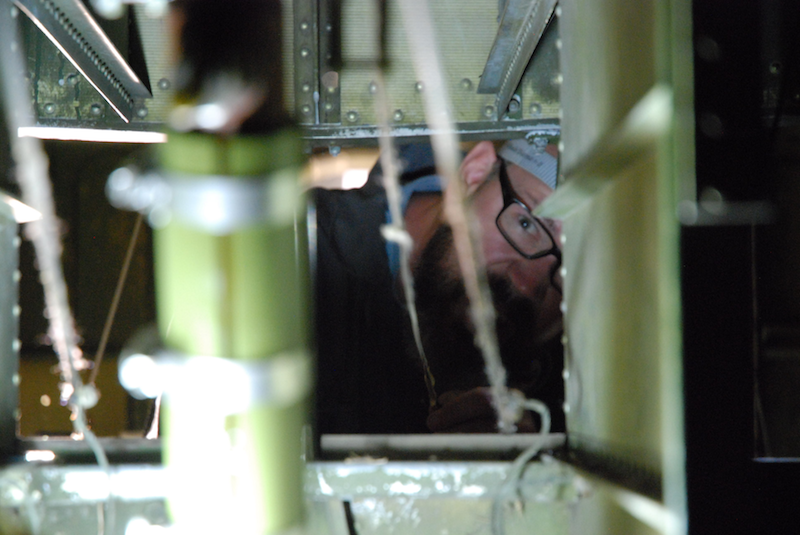
\includegraphics[scale=1.25]{DSC_1156-scaled.png}
%   \caption*{\small \em \color{red} CAPTION NEEDED}
%   \label{fig:stab-one}
%\end{figure}

The work involved in removing flight control surfaces from the ship starts by
disconnecting cables, push rods and torque tubes. These relay pilot input
directly to the airfoil. There are secondary components such as panels,
fairings, plumbing for de-icing boots, grounding straps and electrical conduits.
Finally, when the control surface or stabiliser is ready to be pulled, hinge
bearings and spar bolts must be freed. Support must be provided to the component
once the weight of the assembly is relieved from the airframe. Once
disconnected, the "tail feather" or "stab" is lowered into a cradle on the
ground for cleaning, condition assessment and preparation for restoration. The
approach being that a component is more accessible at ground level than 10-20
feet overhead. Eventually, the outboard wing sections will follow the same
treatment: Not a light undertaking. 

Volunteers on task are comprised of a mix of experienced members and new
additions to the crew. Setting up the scaffold was the first requirement in
gaining access. We had an ex roughneck, Will Assad, building the first tower.
Chris McGuffin, an experienced mountaineer, built the second stage to a full
height of 30ft. Bruce Gemmill donated blood removing the fin retaining hardware,
a modest 64 bolts through 4in. access panels. Peter Trobridge spent some hours
in the hell hole, fitting a tail skid extension jack and running leaders for
control cables. The heat of lights and summer humidity had a therapeutic effect,
much like a sauna. 

Years of battering had taken its toll on the rudder, shearing the torque tube
and stripping the rudder of it's fabric. During this time, generations of
starlings had been introduced to multi-level condo dwelling. Three garbage bags
of nesting material were removed just to gain access to the pulleys in the
vertical stabiliser alone. Starlings are neither good nest makers nor parents to
their young. I will spare you the graphic descriptions of what was removed from
those access panels. 

\begin{figure}[httb]
   \vspace{2em}
   \centering
   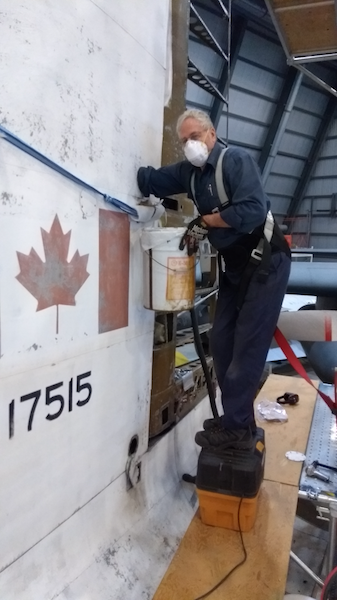
\includegraphics[scale=0.55]{IMG_20180529_132544212-scaled.png}
   \caption*{\small \em Volunteer Bruce Gemmill removing bird nests from the vertical stabilizer.}
   \label{fig:stab-one}
\end{figure}

The horizontal stabilisers were removed earlier, yet there still remained some
nesting material to clear. These assemblies were brought to the restoration
shops for a thorough clean-out and condition assessment. Phil Chrysler, Bill
Cole,  Richard Houle and John Makadi lent their hands at pulling more stacks of
hay out of the two structures. Access proved difficult necessitating  the use of
a hinge rods, in the form of hooked tools for retrieving deep tufts of clumped
nesting. The individual stabilisers were flipped over, blown out, pressure
washed, and oiled, eventually rendering an accessible, stable assembly ready for
restoration. We discovered a large patch on the leading edge of the port
stabiliser. It covered a blunt force impact form which was probably caused by
the boom of a forklift in a former life. 

At the time of going to press, the rudder has been removed from the aircraft and
the vertical stabiliser is slung and ready to pull. The North Star is prepped to
roll out of storage for Canada day and the vertical stab removal is planned for
July 5th. A 30T crane has been rented for the job, with all hands on deck
confirmed for that day's shift schedule. Following this important milestone, the
maple leaf will be lowered from North Star 515, until such time as the
restoration nears its completion. I hope to see the day, dear reader, when the
maple leaf is flown from those heights again.  

%\section{Nr 4 Engine}
%\label{sec:engine_4}
%
%Work has continued on much of the ancillary equipment for the engine. The
%supercharger and intercooler have been completed and installed, as well as the
%reduction gearbox. The radiators and header tank have been restored and painted, and
%two of the three radiator sections have been installed. Restoration work has
%begun on the air intake system, and many of the fuel and oil lines. 
%
%\begin{figure}[htbp]
%   \vspace{2em}
%   \centering
%   \includegraphics[scale=0.5]{"PNS 007-im2".png}
%   \caption*{\small \em Volunteer Peter Trobridge inspecting the air intake fairing from engine \#4 prior to beginning restoration work.}
%   \label{fig:engine_no_4_2}
%\end{figure}
%
%\begin{figure}[htbp]
%   \vspace{2em}
%   \centering
%   \includegraphics[scale=0.5]{"PNS 003-im3".png}
%   \caption*{\small \em Volunteers Robert Desjardins, Bruce Gemmill and Michel Cote hold the refinished coolant tank from engine \#4.  Hours of polishing were required to get the tank to look like new.}
%   \label{fig:coolant_tank}
%\end{figure}
%
%The starter motor was found to be very corroded, and disassembly and repair not viable. A
%new unit has been ordered and will be installed once delivered. The fire
%suppression lines are complete and will be installed along with the cowls when
%ready. Some of the cowl panels have been restored, although it has been found
%that this engine has more corrosion than the other three engines, possibly it
%had been in service longer? This has meant that more work is required to
%refurbish each of the many panels. We still hope to have this engine ready for
%installation by next spring. 
%
%\begin{figure}[htbp]
%   \vspace{2em}
%   \centering
%   \includegraphics[scale=0.5]{"PNS 008-im1".png}
%   \caption*{\small \em Volunteer Garry Dupont working on the re-assembly of engine \#4.}
%   \label{fig:engine_no_4}
%\end{figure}
%
%\section{Fuselage and Main Cabin}
%\label{sec:main_cabin}
%
%With the aircraft moved outside in March, little work was done in the aircraft
%over the winter. Once the temperatures warmed up, we continued work in the main
%cabin to prepare for completion of the painting started last year. Repairs to
%the rear bulkhead are now complete with the installation of several new pieces
%of aluminum to replace corroded ones. A new section of flooring was installed
%where the rear washroom was situated. This required replacing about 1000 rivets!
%
%\begin{figure}[htbp]
%   \vspace{2em}
%   \centering
%   \includegraphics[scale=0.5]{"pns 043-im4".png}
%   \caption*{\small \em A single new floor panel at the rear of the main cabin required over 1000 rivets.  
%   Cleco clips are used to accurately align the panel during riveting.}
%   \label{fig:panel_revets}
%\end{figure}
%
%Cleaning and corrosion removal continued throughout the cabin. It seems whenever
%we feel we are near completion, we find more corrosion. We had also planned to
%finish priming the floor and painting the rear bulkhead before the aircraft
%returned to the hanger later in the year, but this was delayed by the shutdown
%of the project while a new Project Manager was hired by the museum. The wood
%floors and walls still need to be repaired, or new panels made, and all will
%require painting. 
%
%\section{Cabin Liners}
%\label{sec:liners}
%
%All the large pieces of liner have either been repaired or replaced, but with
%limitations on space, most remaining work on the cabin liners has been
%postponed. New window surrounds have also been made, but then all liners will
%require painting and stenciling, and this must wait until there is more room in
%the shop and the paint booth. Liners were also made for the top of the heater
%ducts.
%
%\begin{figure}[htbp]
%   \vspace{2em}
%   \centering
%   \includegraphics[scale=0.5]{P1020369-im5.png}
%   \caption*{\small \em One of the refurbished heater duct sections with a new fabric headliner secured to the top. The sides are covered with mica insulation that was removed, cleaned and reattached after repairs to the metal duct. These will be installed in the main cabin.}
%   \label{fig:heaters_liners}
%\end{figure}
%
%\section{PNS 2017 Update}
%\label{sec:pnsupdate}
%
%We were able to restart work on the aircraft in late January, following the
%arrival of our new Project manager, Rej Demers. So far, we have completed the
%top cowl panels and one of the radiator flaps, which required a repair patch to
%the outer skin, and the electrical harnesses, which are now waiting for
%painting. Work continues on the air box and the remaining cowl panels.
%
%We have decided not to move the aircraft outside this year. With our efforts
%concentrated on completing engine \#4, it is unlikely we would have the resources
%to also complete the repair work in the cabin needed to allow for priming and
%painting, which is the main reason for moving the aircraft outside in the summer.


\begin{footnotesize}
  \raggedleft PNSAC\\
\end{footnotesize}

% End of text.

%%% Local Variables: 
%%% mode: latex
%%% TeX-master: main_document.tex
%%% End: 

